{
\tabulinesep=1mm
 \begin{tabu}{|p{16cm} |}
 \hline
\vspace{2 mm}
\textbf{Ordering and Combinations:} \newline
An important idea of counting is dealing with situations in which all of our choices must be drawn from the same set. Here is a chart which walks you through how to solve problems relating to this idea: \newline
\\
\hline
 \end{tabu}
}

\begin{figure}[!ht]
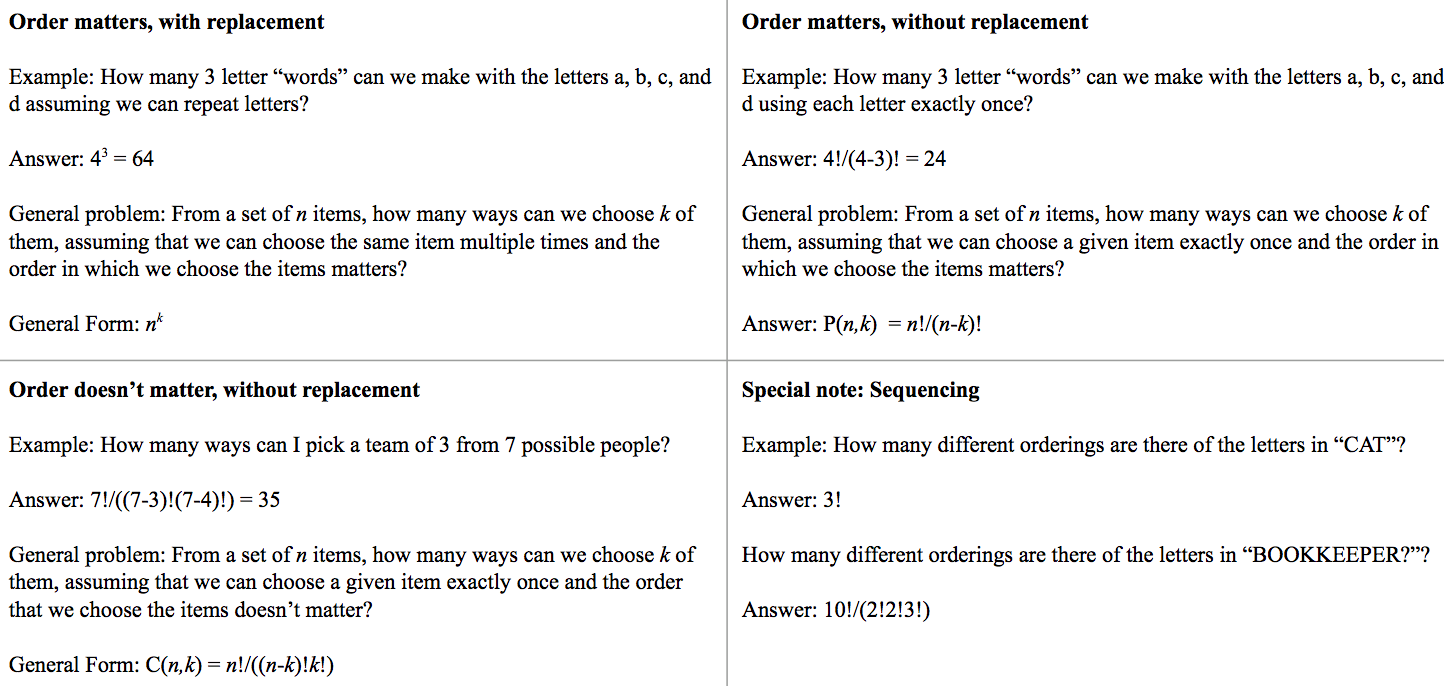
\includegraphics[width=16.5cm, height=8cm]{counting_chart.png}
\end{figure}
